\section{Service Design Methodology}

Below, brief descriptions of five principles of service design are described according to \cite{stickdorn}, together with how the work is divided into iterations, and examples of tools that can be applied.

\subsection{Principles}
\cite{stickdorn} describes five principles that constitute service design thinking, and how to follow these.

He describes how to follow these principles, by making the process user-centered (e.g. via \textit{design ethnography}), co-creative (involve all stakeholders) and holistic (keep the big picture). Sequencing (visualize the service, and make iterations) and evidencing (make the service tangible) are the two last important principles.

\subsection{Sequencing}
Sequencing the process means splitting the design process into iterations, which consists of a number of steps, which are repeated for each iteration. This is a common denominator with the agile methodology SCRUM, which is often applied in software development.

While service design literature and practice refer to various frameworks, regardless of number of steps, every service design project includes: exploration, creation, reflection and implementation \citep{stickdorn}. \cite{expedition-mondial} suggests a model where one iteration consists of insights, ideation, trigger material, and interactions. See figure \ref{fig:iteration}.

\begin{figure}[h]
    \centering
    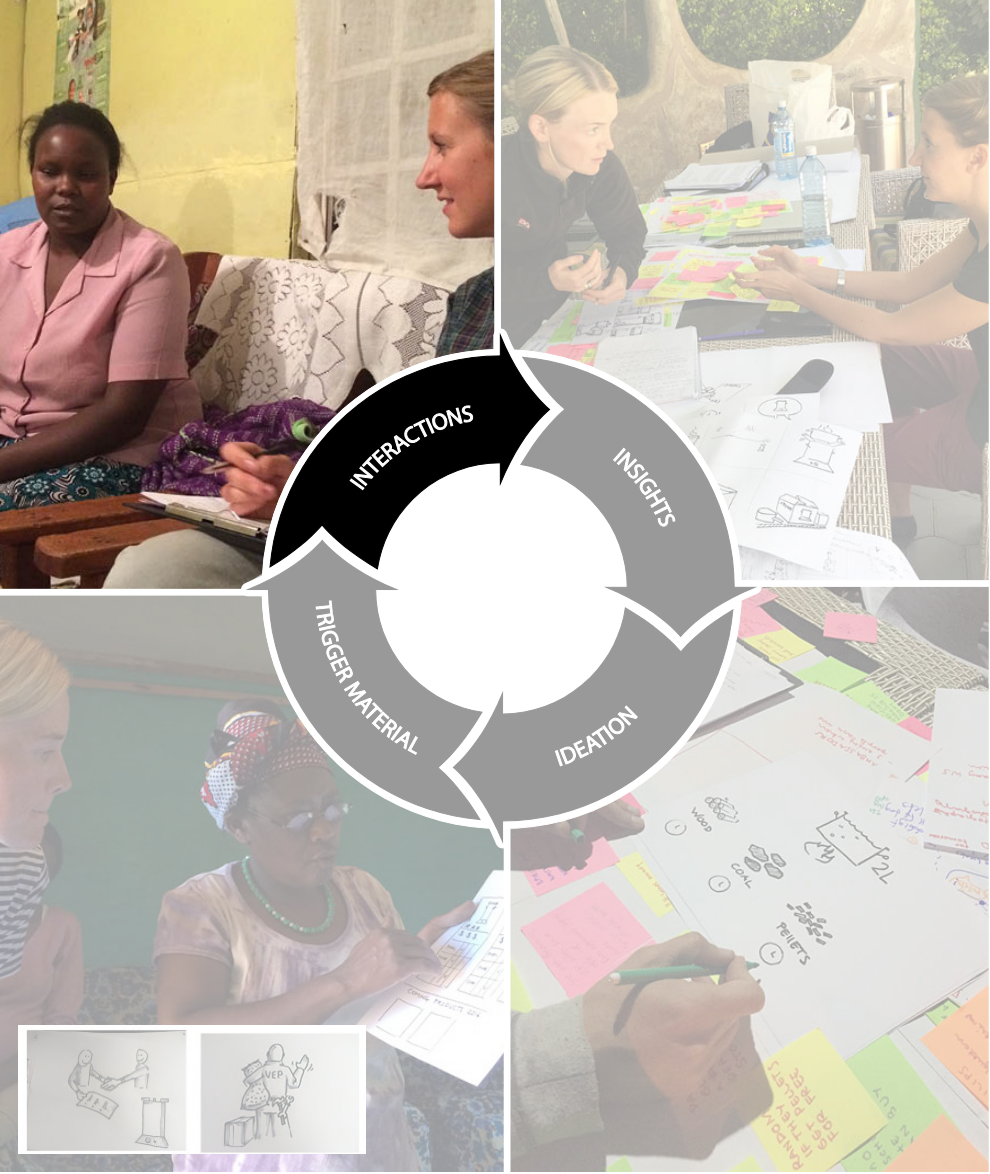
\includegraphics[width=0.7\textwidth]{Iteration.png}
    \caption{In the model by \cite{nissar} an iteration consists of Interactions, Insights, Ideation and Trigger material.}
    \label{fig:iteration}
\end{figure}

\begin{enumerate}
\item Interactions, where you are listening, the \textit{Explorative phase}.
\item Insights, which is where you use the Interactions in order to try to understand, the \textit{Understanding phase}. % better word+
\item Ideation, where you find possible ideas and when creation of new version of the app is done, the \textit{Design phase}.
\item Trigger material, where material is developed to test the outcome of our evaluation in the next round, the \textit{Trigger development}.
\end{enumerate}

The iterations should come closer and closer to a desired outcome. It is not always obvious what this outcome is. For each iteration, the process takes the project closer, from Why? to What? to How?, often with overlaps \citep{expedition-mondial}. See figure \ref{fig:iterationprocess}.

%\begin{wrapfigure}{r}{0.25\textwidth} %this figure will be at the right
%    \centering
%    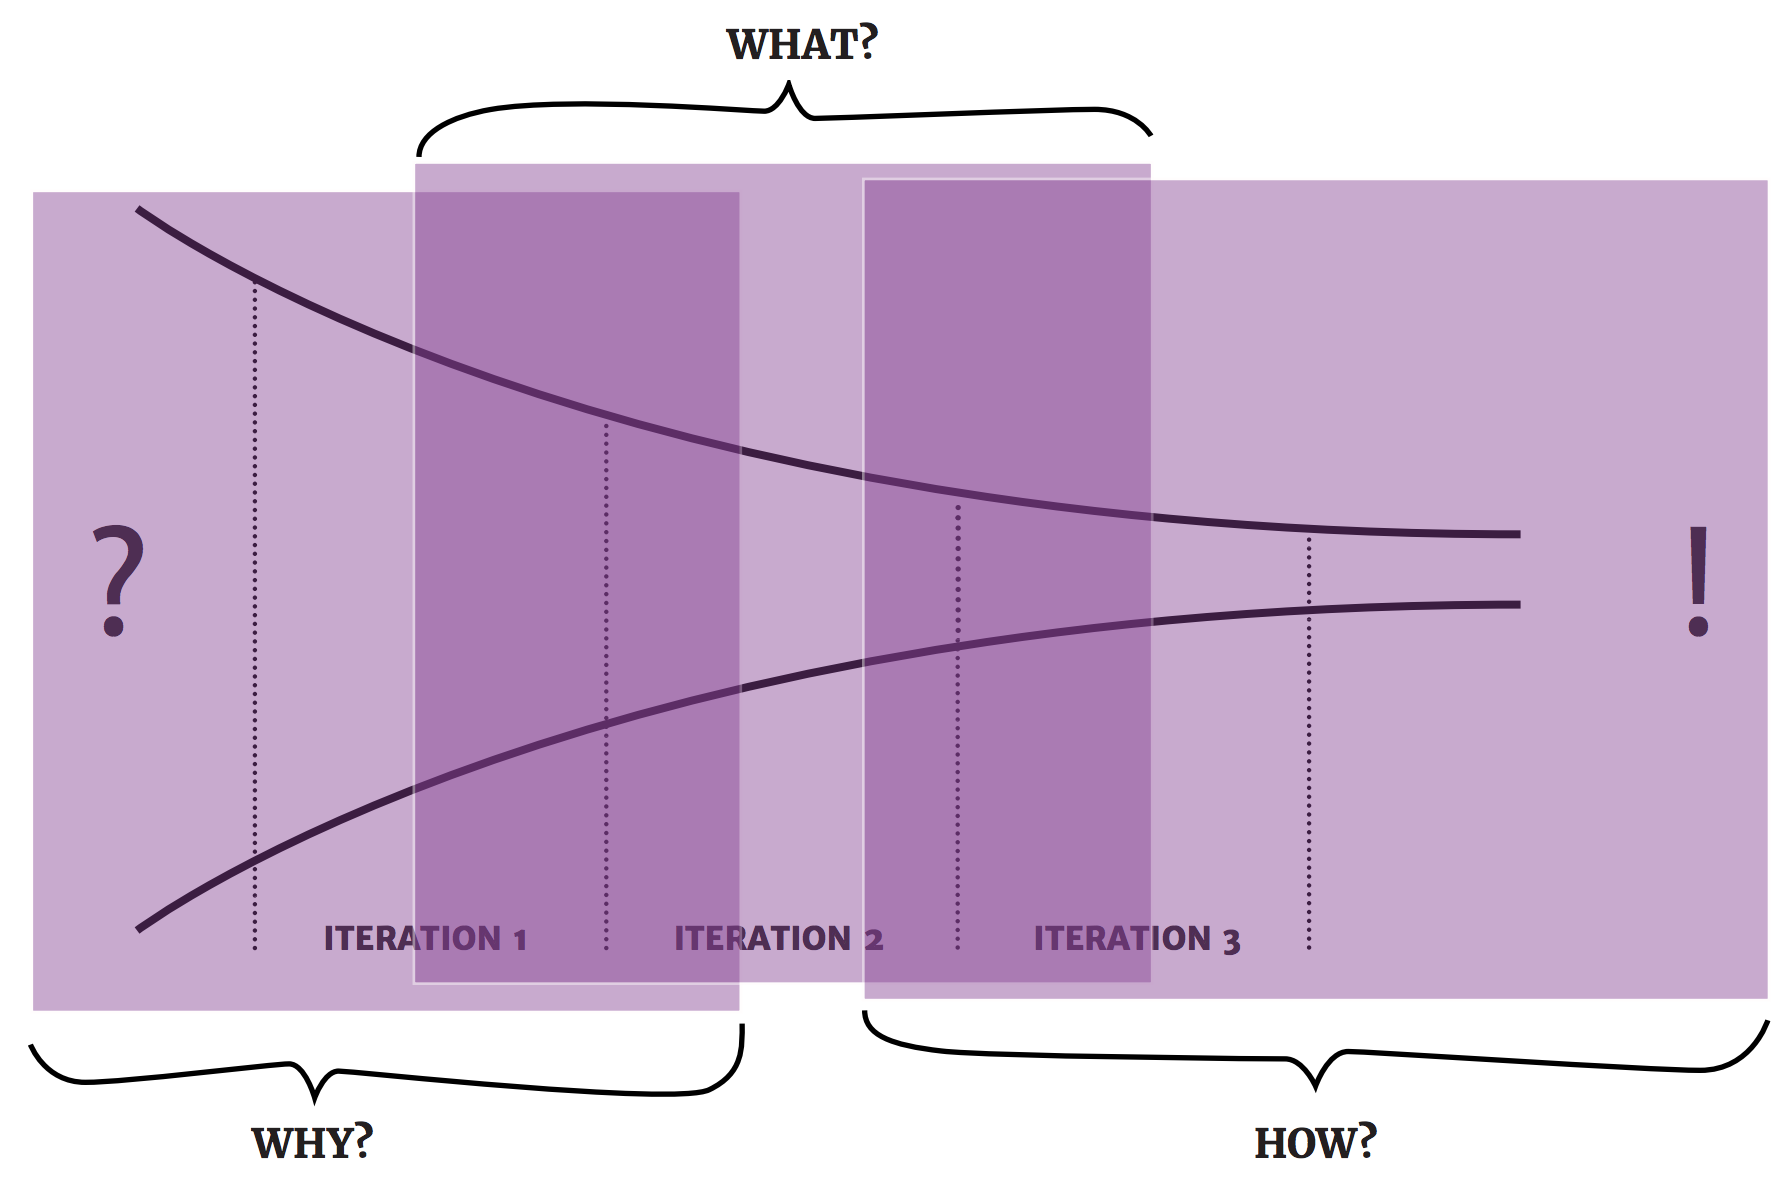
\includegraphics[width=0.25\textwidth]{IterationProcess.png}
%    \caption{Iteration process}
%    \label{fig:iterationprocess}
%\end{wrapfigure}

\begin{figure}[h]
    \centering
    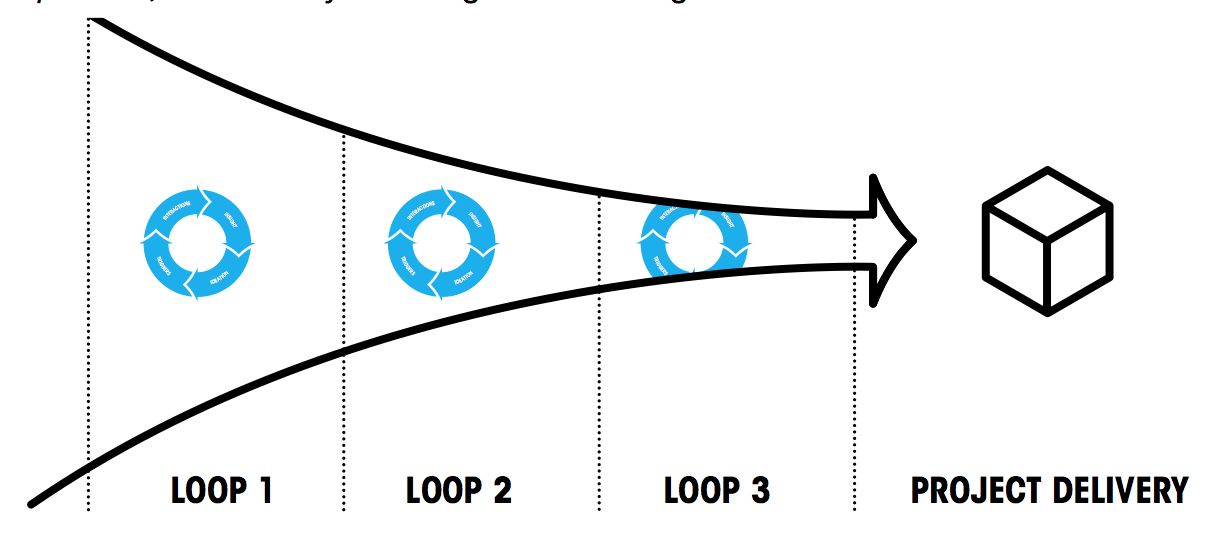
\includegraphics[width=0.8\textwidth]{projectLoop.png}
    %IterationProcess.png
    \caption{The iteration process consists of a number of iterations with different focus, starting with broad strokes, and narrowing down into a concrete product. Between iterations, there is an overlap in "Why?" and "How?", "How?" and "What?", which signals that there is a learning process which means conclusions may need to be quickly questioned as new insights emerge. This is especially important in projects where you work with an unfamiliar target group and there are several uncertainties and constraints.}
    \label{fig:iterationprocess}
\end{figure}

\subsection{Service Design Tools}

There are a number of popular service design tools that follows the five principles, e.g. how to make it user-centered. One is Customer Journey Map, in which an activity (like hosting a youth session) is broken into Before, During and After. Another method is Personas, which \textit{exemplifies} thought users of the app into people with names, having realistic character traits and opinions. The persona's needs can then be thought of when designing. An alternative to Personas are Need groups, where thought users are broken down by their different needs. Instead of designing for a specific person, you design for a person with a specific need. The advantage of Need groups, are that it accepts the view that the same person (Persona) might have different needs, depending on situation. The 5 Why's is a simple method used to dig deep into understanding the interviewee. Variants of the question "Why?"" is repeated five times as a rule of thumb, to understand underlying motives. This method is called "Why-why-why" within interaction design \citep{lowgren}).

Tools to create and reflect can be done via certain work methodology. When you structure and inspire brainstorms, you can ask "What if...?" and do Co-Creation, meaning doing ideation together with stakeholders or users. To create, agile development can be used, which is often suitable for software engineering. The manifesto for agile development is \citep{agile-manifesto}:

\begin{itemize}
\item Individuals and interactions over processes and tools
\item Working software over comprehensive documentation
\item Customer collaboration over contract negotiation
\item Responding to change over following a plan
\end{itemize}

An example of an agile methodology is \textit{SCRUM}, where a project is divided into several iterations similar to a service design approach of sequencing, but also introducing consepts like retrospectives (reflecting on one's work) and sprint demo (demonstrating the results of the iteration to stakeholders) \citep{kniberg}.

There are also some service design best practices: interviews are often done via open questions (encouraging stories) and dialogue can be facilitated with a questionnaire guide. In workshops, post-its are often used, and followed up with specific questions. Service design methodology encourages taking pictures, filming and recording audio, benefiting the analysis done afterwards \citep{expedition-mondial}.

%\subsubsection{Relevancy within Social Innovation}
%\citep{socialinnovation-ehn}

%\subsection{Service Design Thinking}

%\subsubsection{Methodology}

\textbf{The iteration process}

The time in Uganda is divided into three iterations. For each iteration, the result becomes more and more clear. In iteration 1, there is a very broad scope, without digital focus whatsoever, where iteration 2 and 3 gradually introduces the digital solution. See figure \ref{fig:iterationprocess}.

%\begin{wrapfigure}{r}{0.25\textwidth} %this figure will be at the right
%    \centering
%    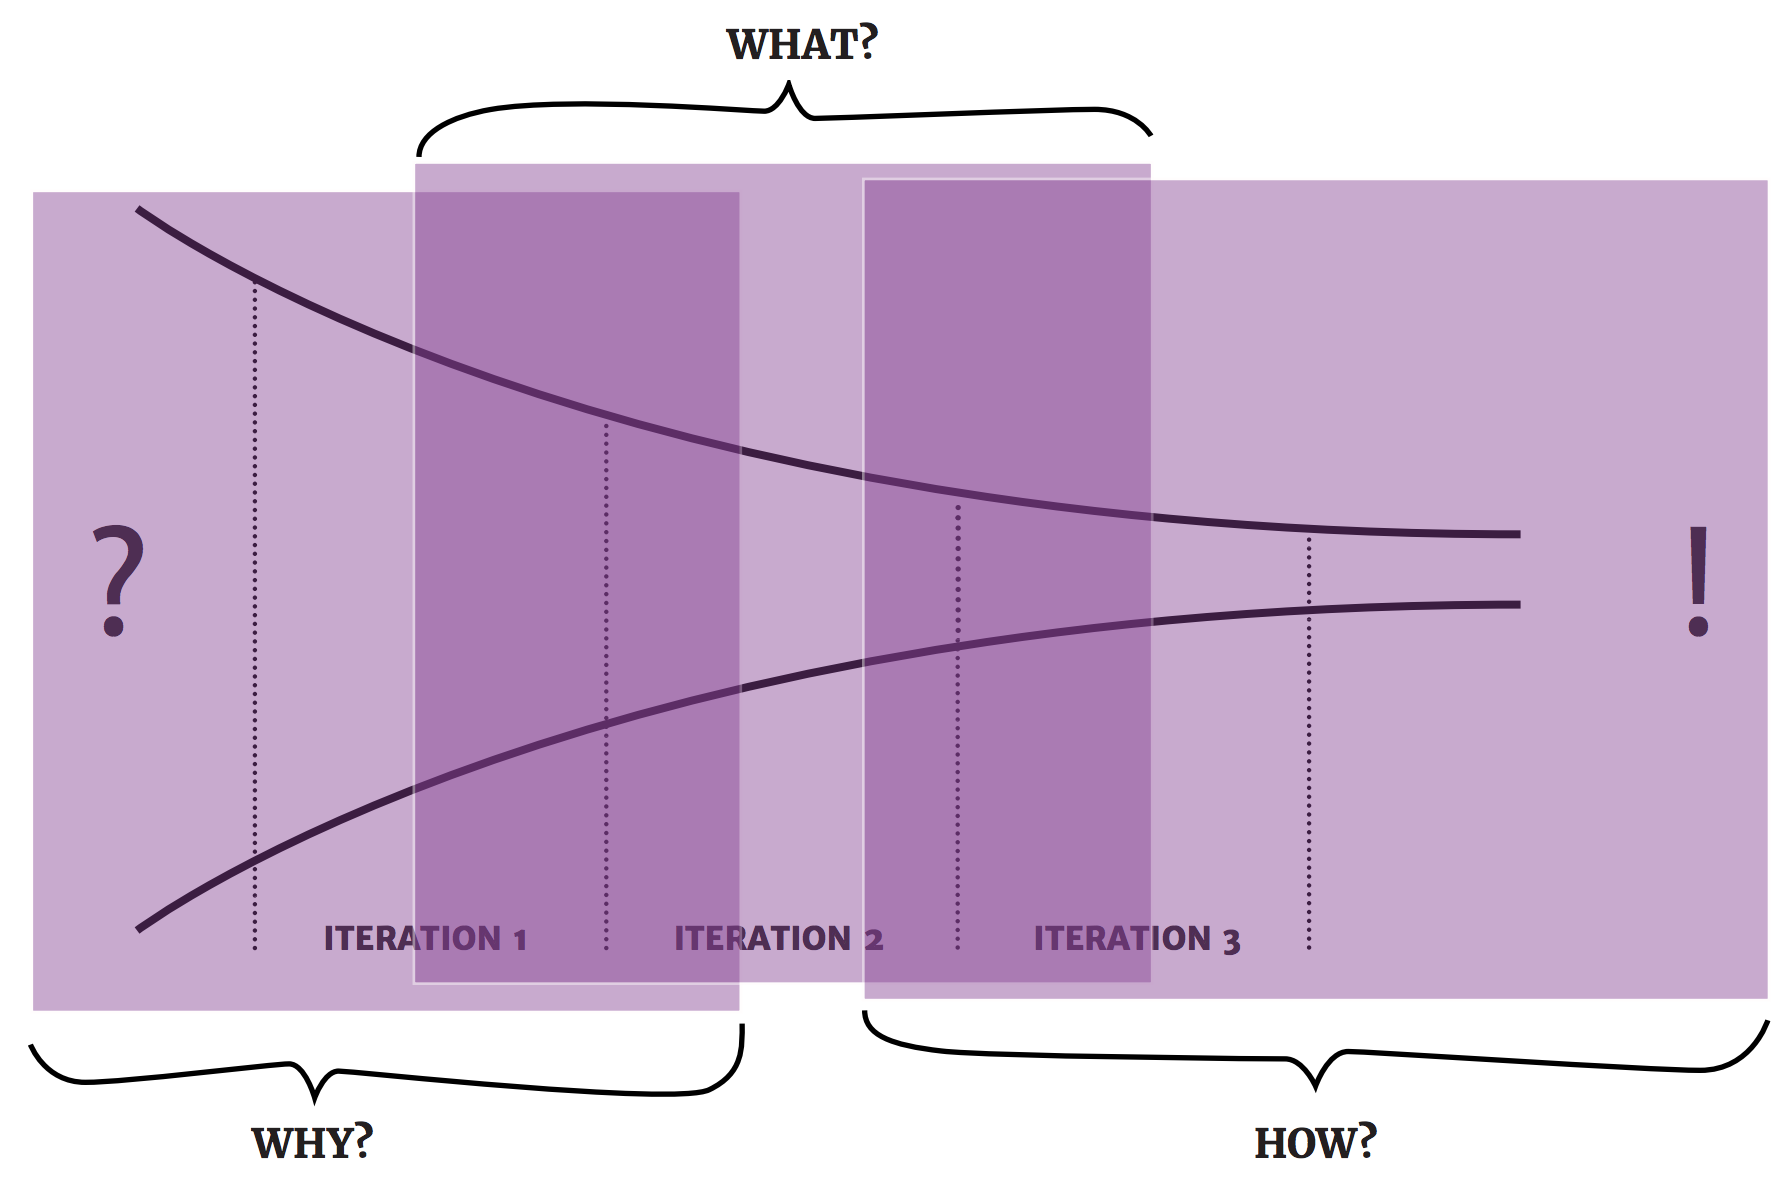
\includegraphics[width=0.25\textwidth]{IterationProcess.png}
%    \caption{Iteration process}
%    \label{fig:iterationprocess}
%\end{wrapfigure}

\begin{figure}[h]
    \centering
    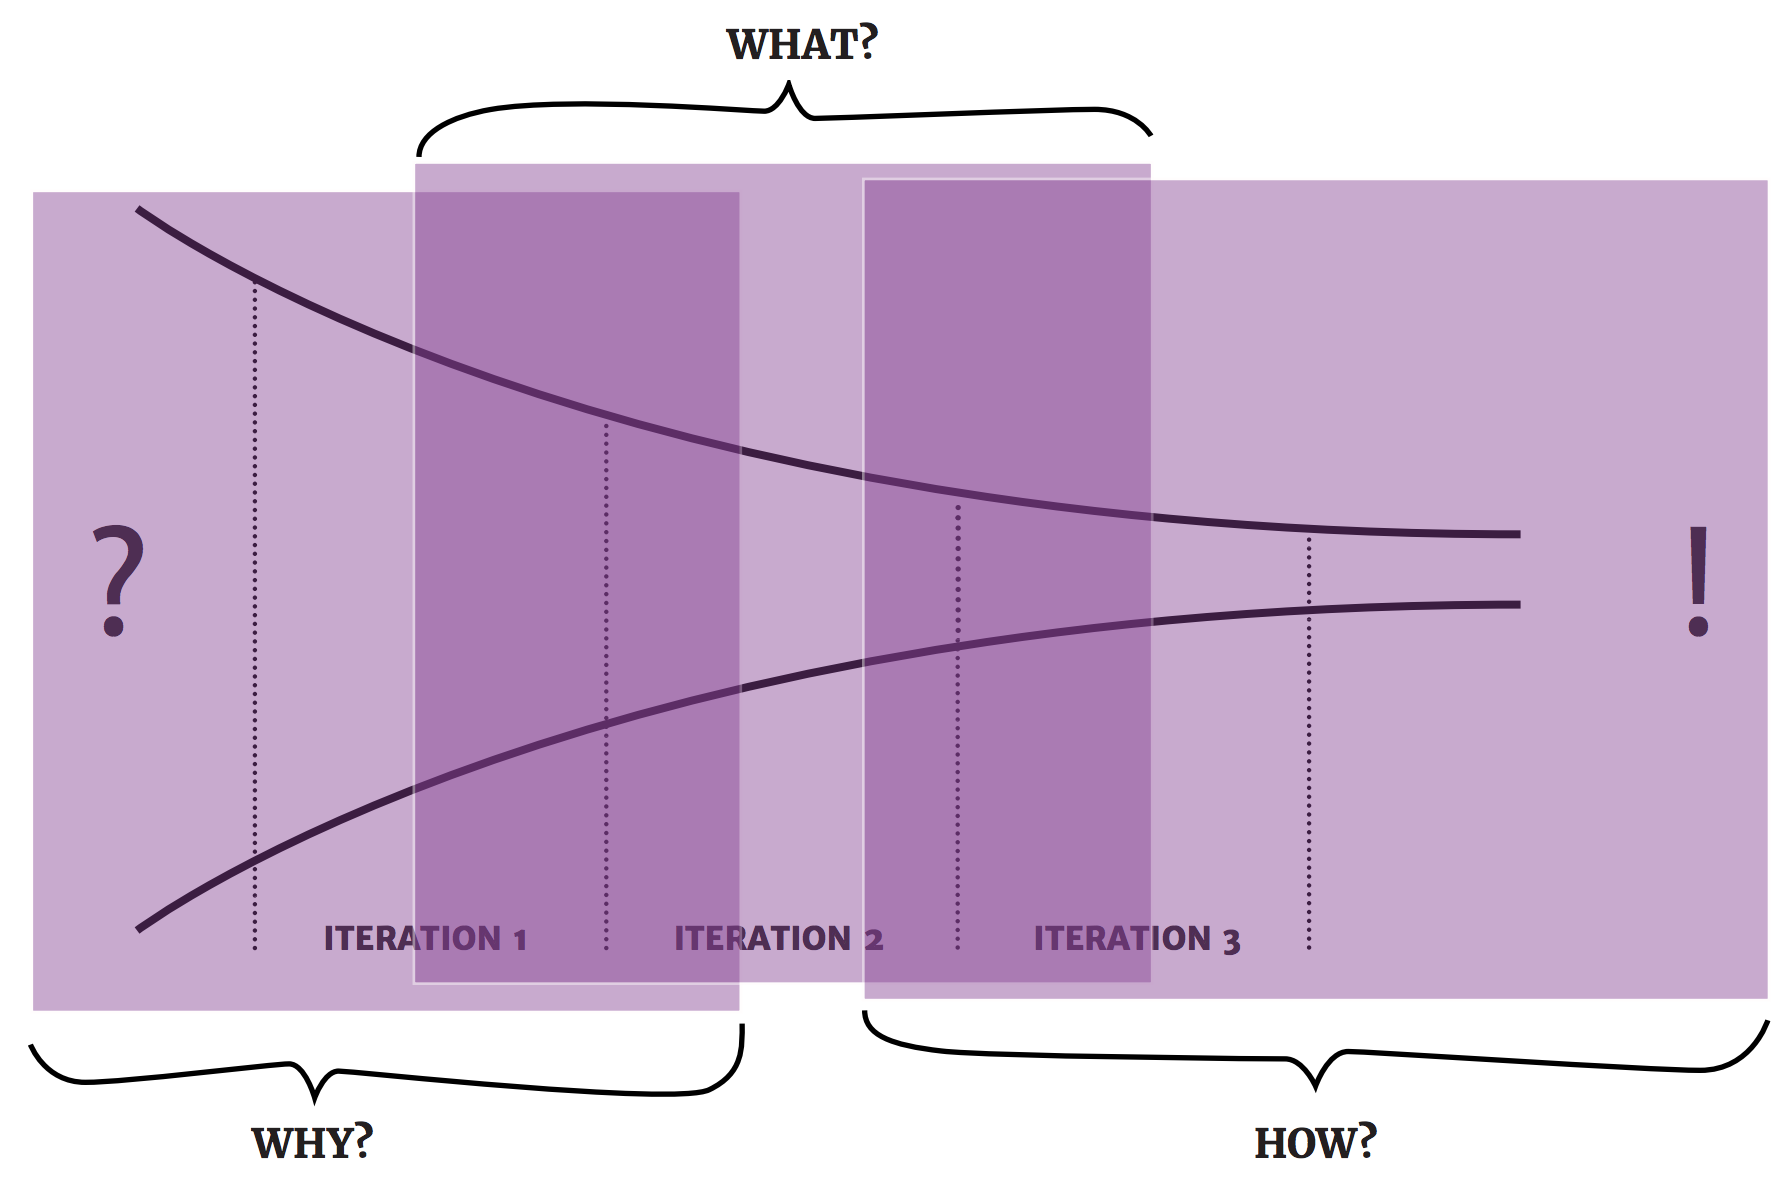
\includegraphics[width=0.8\textwidth]{IterationProcess.png}
    \caption{The iteration process consists of a number of iterations with different focus, starting with broad strokes, and narrowing down into a concrete product. Between iterations, the overlap between "Why?" and "How?", "How?" and "What?", signals that there is a learning process which means conclusions may need to be quickly questioned as new insights emerge. This is especially important in projects where you work with an unfamiliar target group and there are several uncertainties and constraints.}
    \label{fig:iterationprocess}
\end{figure}

\textbf{One iteration} \\
In the way of reasoning around development and design for learning, the steps for each iteration, see figure \ref{fig:iteration}, might be translated into:

\begin{enumerate}
\item Interactions, where you are listening, the \textit{Explorative phase}. 
\item Insights, which is where you use the Interactions in order to try to understand, the \textit{Understanding phase}. % better word+
\item Ideation, where you find possible ideas and when creation of new version of the app is done, the \textit{Design phase}.
\item Trigger material, where material is developed to test the outcome of our evaluation in the next round, the \textit{Trigger development}.
\end{enumerate}

%\subsection{Service Design}
%\citep{servicedesign-ruth},
%\citep{servicedesign-balis},
%\citep{servicedesign-ruth}
%\citep{servicedesign-ideo}
%\citep{servicedesign-stickdorn}

\textbf{The purpose}
Applying service design serves two purposes:

Going from being a computer expert into a socio-technical expert,
In particular, the approach of service design refers to the process of designing rather than to its outcome. (This is Service Design Thinking, 2010, s. 7). ("The outcome of a service design process can have various forms: rather abstract organisational structures, operation processes, service experiences and even concrete physical objects.")

\textbf{The need for service design (in my project)}

\textbf{About service design}
Since service design is a still young and emerging approach, service design education is even younger and just developing. (TISD, 2010)

Without a doubt, you cannot learn what service design is and how to do it just from a textbook. You need to try, fail, learn from your mistakes, improve, try again and thus educate yourself.

Service design education is therefore rather a kind of briefing and tutoring process. Besides explaining the big picture, it is all about giving hints, proposing methods and tools, and showing how to use them while working on a project.

Service design as a practice generally results in the design of systems and processes aimed at providing a holistic service to the user.

Service Design helps to innovate (create new) or improve (existing) services to make them more useful, usable, desirable for clients and efficient as well as effective for organisations.

Service design is all about making the service you deliver useful, usable, efficient, effective and desirable. (UK Design Council, 2010)

(kan lägga till bild)

What distinguishes service design is:

5 principles of service design thinking
Marc Stickdorn
1. User-centred
Services should be experienced through the customer’s eyes. 2. Co-creative
All stakeholders should be included in the service design process.
3. Sequencing
The service should be visualised as a sequence of interrelated actions.
4. Evidencing
Intangible services should be visualised in terms of physical artefacts.
5. Holistic
The entire environment of a service should be considered.

According to TISDT (2010), there is the Customer, Service Provider, Stakeholder, and the Service Designer.

There is then the Touchpoint (every contact point between a customer and the service provider), Service Evidence (a tangible artefact related to a service process), and Service Period (pre-service / service /post-service --current period of a service).

% Här är jag nu i exjobbsrapporten - HÄR

\textbf{How to make it user-centered: TISDT (2010) and Contextual Design (X)}

Agree on a common language!

services are created through interaction between a service provider and a customer. The inherent intention of a service is to meet the customer’s needs and, as a result, be used frequently and recommended heartily. This is often not the case.

Though statistical customer descriptions are important, a true understanding of habits, culture, social context and motivation of users is crucial. We need to put the customer at the centre of the service design process. This requires a genuine understanding of the customer beyond mere statistical descriptions and empirical analyses of their needs. Gaining authentic customer insights includes the application of methods and tools that enable the service designer to slip into the customer’s shoes and understand their individual service experience and its wider context. We are all customers – though with different needs and mindsets. The understanding and disclosure of these disparate mindsets is where service design thinking begins.

we all have individual backgrounds and experiences. The ability to make use of this knowledge during the development of services is crucial for its later success. A user-centred approach offers a common language we can all speak; the service user’s language.

\textbf{Making it co-creative}

This is co-creative.
A broad understanding in various disciplines and a deep knowledge in a specific field is crucial for co-creative work in interdisciplinary teams.


Putting the customer at the centre of a service design process involves facing the reality that potentially there is more than just one customer group, and each group possesses different needs and expectations.
Furthermore, providing services also demands consideration of the various stakeholders,

How can we integrate the stakeholders of a service into the process of designing it?

There are a variety of methods and tools for gaining genuine insights from different user perspectives in the creation of services and for the development, prototyping and testing of these service concepts. This is co-creation, and facilitating this in groups representative of your stakeholders is a vital aspect of design thinking and a fundamental part of service design.

co-creation during the design process facilitates a smooth interaction between the stakeholders during the actual service provision – essential for both sustainable customer and employee satisfaction. Through co-creation customers get the chance to add value to a service in partnership with the service provider early in the development of the service. The more a customer gets involved in the service provision, the more likely this service is of evoking co-ownership which in turn will result in increased customer loyalty and long-term engagement.

\textbf{Making it into sequences} %Chapter: It is sequencing

This is Sequencing.
The series of interactions outline a so called customer journey through the offerings of the respective service.

Imagine a very simple example of a service such as going to a hairdresser. Now try to visualize this service process as
stage play or movie. This movie would consist of a series of static pictures, which would be combined to create a moving sequence. Service design thinking uses this analogy to deconstruct service processes into single touchpoints and interactions. These, when combined, create service moments. Touchpoint interactions take place human-human, human-machine and even machine-machine, but also occur indirectly via third parties, such as reviews from other customers or via print or online media.

Every service process follows a three-step transition of pre-service period (getting in touch with a service), the actual service period (when the customers actually experience a service) and the subsequent post-service period.

Like a stage play, a service moment not only consists of what is happening front of stage, it also includes multiple backstage processes such as cleaning of the shop
33
floor to prepare the front of stage for action. To achieve an excellent theatrical performance, actors have of course to run through many rehearsals; services are no different. We need to prototype services and iteratively test their impact on customers.

\textbf{It is evidencing}

% OBS: korta ner! Ta inte mer så mycket av detta i teorin, för det blir jobbigt att följa upp på.

Make the intangible tangible!

Services often take place unnoticed in the background, like the housekeeping service in a hotel. In fact, services like these are intentionally designed to be inconspicuous. However, if paying a bill is the first moment customers become aware of such backstage service processes, their inconspicuousness might create a disparity in customer expectation and potentially result in their disaffection with the service.

Physical evidence or artefacts such as souvenirs or small bottles of shampoo from your hairdresser can trigger the memory of positive service moments and thus, through emotional association, continue to enhance customers’ perceptions of the service they have received.

Service evidence can thus prolong service experiences beyond the mere service period far into the post-service period. Utilising this effectively has the potential to increase customer loyalty and for customers to recommend the service to others. %Här finns en uppenbart grym koppling till Badass: Making Users Awesome!

In addition, evidence can explain certain aspects of a service touchpoint or process, a sign next to an electric hand dryer pointing out that the proprietor knows that customers would prefer to use real towels but that costs or the environmental impact do not allow this can generate appreciation and empathic engagement.

Evidencing can occur in a variety of forms: bills, mail, emails, brochures, signs, souvenirs or other pro-ducts. These add a tangible component to what would otherwise have been an intangible experience.

Service evidence needs to be designed according to the service’s inherent story and its touchpoint sequence. If a service process is like a movie, a better understanding of the work behind the scenes (i.e. the backstage processes of services) can result in an increased customer appreciation of the service experience.

\textbf{It is holistic}

Keep the big picture!

Which aspects need to be considered when designing services?

the intention should always be to see the wider context in which a service process takes place.

At the level of individual touchpoints and service moments, the focus should be on the environment where the service takes place. The conscious awareness of what customers might otherwise perceive subconsciously with their senses can have a profound impact on the experience of the service itself.

% Detta kanske jag inte tar med?
At the level of the service sequence, there should be a focus on alternative customer journeys. There are always a number of alternative touchpoints and approaches, which need to be taken into account. Sequences change and need to be repeatedly reappraised from various perspectives to ensure a great customer experience. Hence, it is important to map the mood and feelings of all stakeholders throughout the service journey.

To summarise, service design thinking supports the co-operation of different disciplines towards the goal of corporate success through enhanced customer experiences, employee satisfaction, and integration of sophisticated technological processes in pursuing corporate objectives.

\subsubsection{Who are these Service Designers?}

Service design thinking as an interdisciplinary approach includes and connects various fields of activity.

\textbf{Product Design: developing products with service applications (TISD, s. 50)}
This chapter looks at the influences of service production upon product design and considers the implications of the evolution of product designers from designing just products to designing services too.

Design is arguably now focused on the interaction between people and technology, and products serve as platforms for experiences, functionality and service offerings (Buchanan, 2001).

Designers study users and their usage of artefacts to develop better products and generate knowledge that can be embedded into artefacts.

Users generate knowledge through interpretation of this embedded knowledge in artefacts. They need to be able to understand the value, meaning, and the ways to use the artefact in different situations of their daily lives.

\subsubsection{This is co-creative}

The concept of activity refers to participants’ interactivity, initiative and style of collaboration and contribution in design events. User roles may vary from proactive participation where users contribute to solving and framing design challenges to passive roles where designers instead interpret user data without any direct engagement with the user community (Keinonen, 2009).

\textbf{Iterative design development} helps to solve problems found in user testing. There must be a cycle of design, testing and measurement, then redesign, repeated as often as necessary. This is a way to incorporate results of behavioural testing into the next version of the system. Making a system user friendly and easy to operate is the goal of this approach (Gould and Lewis, 1985). Iterative design is a design methodology based on a cyclical process of prototyping, testing, analysing, and refining a work in progress.

Both conceptual and iterative design approaches are important phases in the service design process. The challenge is to design user-orientated hybrids that incorporate both the customer facing products and that help articulate the service they assist in offering.

\textbf{Product-service hybrids}

Koivisto (2007) defines hybrid products as products where the service has been designed as an inseparable part of the product. % A good example of this is Apple’s iPod and iTunes product package (Apple, 2010). Developing such a hybrid product means that both the product concept and a service system are developed in tandem.

A successful service design project requires integrating stakeholders as earlier as possible in the project development process. Opportunities to iterate the product development process together with the stakeholders involved in the project should be created as soon as possible. This will in all likelihood result in an increase in proactive solutions. Management buy-in needs to be secured to support the process. There has to be constant communication, continuous sales work and partnership with the designers.

\textbf{Creating value propositions with users}

Mark Jones, Lead of Service Innovation at IDEO, says that from his perspective the design process begins with understanding the product’s context of use, and observation of users’ experiences by moving into the field to observe users and how they interact with the product. In a typical development project pre-research, work is done before one or two workshops with the stakeholders. Subsequently, the development case needs up to six or seven iterations and mock-ups as part of the iterative product development process.

Typically, a design team would consist of an engineer and designer. When you start designing actions, systems or product service systems, this range of expertise needs to be expanded through the involvement of a human factors expert. Design’s role is to illustrate and represent the complexity of the system to make it more understandable as well as represent the added value that the product brings to the company. Participatory design methods are used in the development work and this involves relating extensively with clients. How the methods are chosen depends on the business case.

% Detta går att diskutera under Future work, om att Plan vill använda verktyget till fler utbildningar, eller att YoungDrive vill bli ett socialt digitalt företag
When the product service systems or service-product hybrids are developed it’s not only about what kind of services are co-created with users but also about what the service’s role is within the organisation’s business model. When designed and considered well, the product service systems and service-product hybrids detailed here can make key contributions to the overall value proposition and desirability of the products offered by an organisation.

\subsubsection{Graphic Design: providing visual explanation}

Mental models help an individual’s orientation in the world; they are the abstract and reductive mental representation of the complexity all of us face in everyday life – the schemas by which all of us understand the world around ourselves.

%Koppla såklart till deras digitala kunnande
If, however, a user is confronted with a situation they have never previously experienced, they cannot fall back on an existing model.

The metaphor of the online shopping cart for example, promotes the development of a new mental model, through reference to an analogous experience. % The individual can draw upon known mechanisms and functionalities associated with, in this case, shopping carts to understand a novel and largely intangible online system of payment. Even though online shopping is phenomenologically different from previous experiences the user might have of “offline” shopping.

It is the graphic designer’s task to trigger an individual’s apriori mental models, or at least to positively influence the accrual of such cognitive representations of meaning.

This chapter explains what graphic design is capable of and what role it can play within service design – from the perspective of a graphic designer.

Two tasks: information and branding

% D.v.s., viktigt accosiera med YoungDrive, som de litar mycket på
Branding refers to helping an offering establish a visual identity and familiarity in the eyes of customers. Thus graphic design taps into and adopts a number of patterns of which the customer already has a mental model: use of the colour green in packaging can, for example, suggest an association with the user’s ideas of freshness, organic products or, more recently, environmental friendliness.

Information design, on the other hand, pertains to the task of making complex and abstract content accessible in a simpler way. Through logical composition, visual hierarchy and the use of visual metaphors, viewers are supported in their absorption and comprehension of information.

Branding supports the customer to emotionally approximate himself with the theme or emotional context of the experience.

Within this setting, information design leads to a satisfactory and positively associated user experience.

 It may be forgivable for a customer that their bank’s corporate identity does not really inspire confidence, but they become upset when they cannot see their balance because the pixelated letters on a screen are too small to read.

Visual presentation plays an important role in three ways. It pre-empts the actual service process, it controls customer expectation, and it can promote trust during interaction. The so-called look and feel can evoke a positive prevailing mood, or even makes the service usable in the first place through visual aides. Lastly, the visual appearance acts as an anchor that links the user to the positive experience. Visual control is henceforth a key competence in the conception of design propositions.

\textbf{Visual control}

For graphic designers it does not matter if they are working on a product or a service offering. Whether they have to create a print product, an interface or a three-dimensional presentation, it is imperative for the graphic designer to know what they want to offer the customer on a visual level, in order to adequately convey the thoughts and concepts standing behind the design proposition.

%It is nonetheless important to understand that the role of a graphic designer does not lie in sticking a previously developed logo on each and every surface. The complete visual appearance consists of far more factors than just such signage. The use of colours, text, photographs, the chosen medium, the type of production – there are countless ways to keep an image consistent and also countless ways to dilute it. As many parameters decide what is told by whom, as how it is told.

%The orchestration of these factors requires
designers to be open to current trends and familiar with previous trends to best enable them to understand the world of their target audience.

Branding and information design complement each other in a symbiotic way. Function and emotion combined define the concrete parameters like typography, colours, form and composition.

\subsubsection{Interaction Design: services as a series of interactions}

Services are a series of interactions between customers and the service system through many different touchpoints during the customer journey.

To value your customer, you need to spend some time understanding the interactions they have with your service, and that means two things. Firstly, viewing your service through the customers’ eyes, and secondly, designing in such a way that customers receive consistent experiences over time which they consider valuable. It’s strange, but repeatedly we see companies ignoring both of these aspects, with the consequence that customers feel ignored and value is lost.

digital interaction is an area that is becoming more and more central for service delivery.

\textbf{Desirability is king in the land of interface design}
% Desirability in a service fires desire in the customer. Desirable interactions are something you tell others about and which give trust with, and loyalty to, the service. Finally, and this is becoming more and more important, desirability has a strong emotional dimension, often giving a pleasurable experience from the interaction.

it’s not an easy thing to do, mostly because desirability requires collaboration across traditional silos in a service organisation.

\textbf{Utility - it just has to work at a functional level}

scoring highly in terms of utility demands that you really understand your customers and their needs, together with an understanding of the functional benefits of your design offering.

To get a high score on the utility level you need to offer people what they need but no more and this is not always an easy thing to pull off. There is a big tendency for feature creep in interactive services – hey let’s add that feature, it doesn’t cost extra!

This leads to a service that has strayed from the core offering and which customers find vague or fuzzy. Utility is about what your service does.

\textbf{Usability - Keep it simple, stupid (KISS)}
While utility is about what, usability is about how. Usability is all about how easy it is to get to the offering (utility value) when using the service.

It’s all about ease of use, which often relates to how quickly and smoothly a customer can move through the service journey, and the risk they run of misunderstanding something and making errors (and error recovery of course). Its key metrics are time, errors and flow.


Usability relates strongly to how the interaction is strung together, often in terms of the design of the dialogue between the (online) service and the customer. Within interaction design, this is often termed the interaction architecture, and describes the functional divisions between the different parts of a website, and upon the functional layout of a page. A website needs to be structured according to the customers’ expectations of structure. This is described as the customers’ mental model, and ideally, your website structure should mirror the customers’ mental model.

\textit{A good means of finding the customers’ mental model when designing a service is to ask customers to structure the site for you, and there are several methods available to help them do this in a structured way.}

% Väldigt bra innehåll, som hjälper mig!
There are three keys to unlock the door to usability: \textbf{frequency, sequence and importance}. Frequency says that things the customers do most frequently (e.g. next, back, search etc) should have a prominent position in the sequence. Sequence says that activities that occur in sequence should be presented in sequence (i.e. you pay at the end of a transaction, not in the middle). Importance means that important pieces of information need to be given clearly and at the right time (e.g. if you only ship within the EU, then a customer trying to buy from India needs to know this early on – not at the end of a six-page check-out dialogue). Understanding the customers’ mental model and applying the frequency, sequence and importance rule will crack most of your usability needs. But, beware, like all rules, you cannot follow them blindly, and there are always tradeoffs that have to be made between these elements.

\textbf{Pleasureability - the pleasure principle}
We like things that make us feel good. In fact, we use a lot of time, effort and money on pleasurable things. Why is it, then, that when it comes to digital interactions, most of it is designed to be neutral at best?

It’s as if we have all been brainwashed to expect utilitarianism in everything digital. Luckily, we are entering into the experience economy, in which, finally, pleasurable experiences are recognised as central in today’s markets.

Pleasurability is about how the whole solution makes you feel.


It relates to a sum of details within your service, and often relates this to culture from the world outside. Pleasurability relates to the way the interaction is designed. The way it looks, the way things move, the feedback it gives you. It relates to style, but it also relates to much greater things. It relates to your brand and to what people expect from you. Pleasurability is not something for everyone. Ryanair, for example, is fo-cussed upon the utilitarian value and explicitly distances itself from highbrow style in their interaction design, with great success. It focuses upon utility and usability as part of its utilitarian approach, and this links to its no-frills offering very well.

A high level of desirability requires strong internal alignment, a strong brand and knowledge of managing design. However, it is a very strong differentiator and gives a mind share amongst customers.

%Limitations: don't to this, it's too hard, and takes too long time
\textbf{Desirability – moving from good to great}
If you put some effort into your interaction design you will be able to make a perfectly good solution, but if you are searching for true desirability you need to work hard. The benefits can make it worth it, but you have to be very confident of your offering, your position, and have a crystal-clear brand to be able to move up the desirability scale.

\textbf{Conclusion}
To conclude then, it’s time for you to think about the mix of utility, usability and pleasurability that fits your service. The answer to this lies in understanding your customers, your offering and your brand strategy and in finding an alignment between the interactions you design into your service and what your company is all about.

\subsubsection{Social design: delivering positive social impact}

% Det här är bara en sidonot, men om en designstudent skulle stå i sitt bås och faktiskt *designa* under tiden, skulle det nog få väldigt mycket uppmärksamhet! Som en pop-up store.
% From this perspective, there is much to query and explore in the broader role of design disciplines and how they are positioned alongside other disciplines. Designers possess more than simply an ability to style products; they are practitioners of an applied process of creative skills: identifying problems, researching, analysing, evaluating, synthesising and then conceptualising, testing and communicating solutions. Design, whatever the discipline, is not only about an end product, but rather a systematic process of identifying problems, then researching, creating, testing and implementing solutions.

One can look to the design profession for inspirations on style, but further investigation will show that design offers more than solely the creation and promotion of consumer goods. It is also possible to observe that designers have, through their broad and adaptable skill set, a service to offer to all areas of society. Such broader applications of design have variously been termed \textbf{“innovation”} %Snygg brygga till innovation!
and “design thinking”, two terms that have seen David Kelley’s IDEO and D-School gain kudos in the pages of Business Week.

Employing the design process to tackle a social issue or with an intent to improve human lives is known as social design.

Methodologies of co-design, social innovation and service design have dramatically broadened the application of “design thinking”, giving impetus and stability to a social design movement. One could argue that through these new methodologies, designers are better communicating the value of their creativity.

Recognising the growth of a potential new design movement, many designers have begun forging multidisciplinary networks with the aims of social improvement through design.

\subsubsection{Technology in service design}
At McDonald’s, technology was extensively used in the front office to guide, monitor and control employee behaviour.

However, the McDonald’s employee, no matter how callow, continued to be an important touchpoint for customers, just as he or she is today at Starbucks.

With the growth of computer and communications technology, service design took another leap forward in the pursuit of efficiency by substituting technology for direct customer-employee contact entirely. Of course, we can point to early examples of self-service technologies such as the vending machine (invented in the 1880s in England) or the cash machine (invented in the 1960s), but these required the customer to be physically present at a site designated by the service provider. However, the invention of the web, which popularised the use of the internet, revolutionised services, since the service provider, such as Amazon, could be located anywhere in the world.

\subsubsection{Design ethnography: taking inspiration from everyday life}
Design Ethnography is aimed at understanding the future users of a design, such as a certain service. It is a structured process for going into depth of the everyday lives and experiences of the people a design is for. The intention is to enable the design team to identify with these people, to build up an empathic understanding of their practices and routines and what they care about. This allows the team to work from the perspective of these users on new designs for relevant slices of their daily lives. Designers use this understanding to work on idea generation, concept development and implementation.

Ethnography is a research methodology developed and used in various social sciences such as anthropology and sociology. Its literal meaning is “description of people”.

\textbf{Firmly rooted in the design process}
Design ethnography is ethnographic qualitative research set within a design context. It delivers results that inform and inspire design processes, for instance service design processes. It offers reference material on people’s everyday lives; \textbf{their practices, motivations, dreams and concerns.}

Design ethnography allows the team to work from the perspective of these users on new designs for relevant slices of their daily lives. Designers use this understanding to work on idea generation, concept development and implementation.

\textbf{Key role in service design}

Service design is a very wide field that encompasses many disciplines, not only the various expertises of design, but also other disciplines such as strategy and technology. The teamwork between these disciplines needs a shared focus and language. The results from design ethnography facilitate that focus and language by offering a firm reference point that connects all the disciplines involved – the people they are ultimately developing the services for. This is relevant not only during the design stage of services but also during implementation. Design ethnography helps to communicate concepts, guidelines, strategies, scenarios and the like to people throughout companies.


You must engage with the hearts and minds of people if you want to design successful and popular services. You cannot really do service design without some form of design ethnography. The level of detail of the ethnographic research can vary greatly between projects (depending on time, budget and experience).

In small-scale projects it might be just a few days, while in large-scale projects it can take several weeks.

Service design is an inter-discipline where T-shaped people collaborate. The concept of T-shaped people was introduced to the design and innovation field by the design consultancy IDEO (Kelley, 2000). The idea behind the metaphor is to indicate that most professionals have both a deep expertise in a given field and a broad understanding of other fields they encounter in their work. In strategic and innovative projects, as many service design projects are, various T-shaped people with different backgrounds and roles are working together as part of the same team. This is both true for the agencies involved and the team members from the client organisation.

This is co-creative.
A broad understanding in various disciplines and a deep knowledge in a specific field is crucial for co-creative work in interdisciplinary teams.

There is usually a notable overlap between the various specialists. That is why and how they understand one another and are able to collaborate. Without the deep expertise of these various specialists, the knowledge and skills in the service design team would be very shallow. Generalists who know a bit of everything cannot make a real difference in service innovation.

The methods used during the development stage contribute to idea generation, concept development, co-creation, prototyping and validation.

\textbf{The Tools section} in this book offers detailed descriptions of many of these methods. Throughout the research and development process, design ethnography offers a bridge between the service users, the service providers and the service designers.

\textbf{Synergy between design and ethnographic research}

The empathic conversations between the various people and parties involved require both a sensitive attitude and a strong, visually engaging approach. The research activities and materials need to be well designed in order to get people involved and elicit useful and inspiring results. And the subsequent new designs need to be researched again, to make sure that the final results will be further improved in an iterative process. In this way service design not only takes inspiration from everyday life, it puts it at the very heart of the design process.

\subsubsection{Tools of service design thinking}

It is an iterative process
Marc Stickdorn outlines a reiterating four step approach for designing services.
AT-ONE
Simon Clatworthy presents an example of a service design workshop series.
This is a toolbox – not a manual
With the help of the service design community, STBY describes a collection of service design tools.
This second part describes how service design actually works.
The first text explains the service design process along four iterative stages and the difficulty to define a standardised procedure to design services. The subsequent article however introduces an example for a rather structured approach for the early phases of a service design process. In the following a toolbox of 25 service design methods and tools are illustrated and assigned to respective process stages.

\textbf{It is an iterative process}
Exploration
Creation
Reflection
Implementation
(kan lägga till bild)

\textbf{The iterative process of service design thinking}

(lägg till bild, s. 117, "The Squiggle")

Although design processes are in reality nonlinear, it is possible to articulate an outline structure. It is important to understand that this structure is iterative in its approach.

Although design processes are in reality nonlinear, it is possible to articulate an outline structure. It is important to understand that this structure is iterative in its approach.
This means that at every stage of a service design process, it might be necessary to take a step back or even start again from scratch. The single but very important difference is in ensuring that you learn from the mistakes of the previous iteration. Thus, the proposed process is just rough framework and should not be considered a prescriptive, linear how-to guide. In fact, the very first step of a service design process is to design the process itself, since the process ultimately depends on the context of the service being designed and thus varies from project to project.
The iterative four steps of exploration, creation, reflection and implementation are a very basic approach to structure such a complex design process.

% Detta går att ha med till Diskussion, att jag inte hade tänkt ha en så tydlig design-process från början, men att Service Design hjälpte mig så fort det introducerades, och att det var extra viktigt då det fanns så många osäkerheter
“Designers need to be critical towards any theory or model of a design process” (Hegeman, 2008). With this acknowledgement it is perhaps also worth noting that whether the process is intentional or not, it will assume a significance upon the final design outcome. The benefit of clearly articulating the design process is that it enables a greater degree of reflection upon the influence that the designer has had on the designed outcome.

The iterative four steps of exploration, creation, reflection and
implementation are a very basic approach to structure such a complex design process.

% Literature and practice refer to various other frameworks made up of three to seven or even more steps, but fundamentally they all share the same mindset (Best, 2006; Mager, 2009; Miettinen & Koivisto, 2009). The wording also varies: identify-build-measure (Engine, 2009), insight-idea-prototyping-delivery (live|work, 2009), discovering-concepting-designing-building-implementing (Designthinkers, 2009), to highlight just a few.
%PS: jag tror att den ena av dessa är MVP, Engine, 2009

When considering the design process it is important to keep a few fundamental considerations in mind. It is necessary to make recurrent leaps between designing in detail and designing holistically. This means that whilst working on the details of a touchpoint you need to keep in mind where that touchpoint sits within the whole customer journey, or when working on redesigning employee interactions you need to consider the organisational structure as a whole. Furthermore, you will always have to cope with dilemmas and paradoxes. Since you cannot pay attention to every aspect, insight or point of view, you will have to make decisions according to your budget, resources and the views of your clients.

%  Like a chain that will break at the weakest link, the customer experience will break at the weakest touchpoint. (s. 131)

(lägg till bild The Double Diamond)

\textbf{Stage 1 - Exploration}

This stage is all about discovery. Service designers will be trying to discover new perspectives on a particular service. This could involve stepping into the shoes of customer, staff, managers, or even rivals, in order to develop new insights into the service experience. As this will form the foundation for the rest of the project, it is crucial that the tools used generate both intimate and engaging results. (s. 141)

Although service design aims to put the customer at the centre of its process, the process seldom starts with the customer.

The first task of a service designer is to understand the culture and goals of the company providing a service.

Furthermore, the process starts by identifying the problem a service designer should work on; this problem is usually an organisational one or is initially viewed from the organisational perspective. It is important to understand the company’s point of view on a certain problem, and in fact it could be argued that much of a service designer’s role is in articulating the organisational problem from the perspective of the customer.

% Sprint #1! Utan Expedition Mondial hade detta aldrig hänt: "What's it like being a coach?". Jag hade gått på vad min uppdragsgivare sagt till mig.
The second task is not finding a solution, but instead iden-tifying the real problem. Gaining a clear understanding of the situation from the perspective of current and potential customers of a certain service is crucial for successful service design. Again, it is important to keep the big picture and as far as possible ascertain the true motivations behind customer behaviour. To this end, it is important to look for insights beyond simply gathering of empirical data. Service design uses a vast collection of methods and tools from various disciplines to explore and understand the behaviour and mindset of all people involved. Ethnographic approaches from the social sciences have thus been adopted as one of the most commonly employed research approaches in the design of services. Put simply, it is not about trying to find the solution immediately – it is about finding the problem first!

Gaining a clear understanding of the situation from the perspective of current and potential customers of a certain service is crucial for successful service design.
The third task is to visualise these findings and as far as possible the underlying structure of the previously intangible services. This helps simplify complex and intangible processes and promotes a sense within the design team and amongst the service stakeholders that it is possible to change aspects of the service proposition that might not appear to be functioning appropriately. Again, there are numerous methods and tools from various disciplines that can be adopted to assist this.
% TODO: visa Iliana min bild, customer journey

\textbf{Create \& Reflect}
Creation is where insights are visualised into new ideas and concepts, while reflection involves testing these ideas and concepts to find out how they can be further improved. Holistic solutions require the involvement of a wide range of stakeholders, and thus many of the creative tools here are designed around bringing as many people as possible into the creative process. The tools for reflection allow the ideas for solutions to be developed into prototypes, and tested against the insights generated in the exploratory phase. (s. 141)

\textbf{Stage 2 - Creation: Concept design}

One of the main features of service design thinking is that this
approach is not about avoiding mistakes, but rather about exploring as many as possible mistakes.

%Detta talar för att jag faktiskt ska ha tekniskt lik workshop redan i del 1
The crux is to make them as early as possible in the process and learn from these as much as possible before you implement or adopt the new concepts.

The cost of an additional iteration during the concept design stage is marginal compared to the cost of failure with this concept after its launch.

sticky-notes are a simple and quick tool to visualise processes, illustrate associations and relationships or provide mnemonics during co-creative ideation pro-cesses.

Sticky-notes provide a visual support to keep track with this quick and iterative approach to development. The task is to generate and develop solutions based on the identified problems and in-depth insights generated in the exploratory stage; the identification of customers’ needs, motivations, expectations, the service providers’ processes and constraints, and the illustration of the customer journey, consisting of a sequence of touchpoints.

In order to achieve holistic and sustainable solutions it is crucial to include all the main stakeholders and work with interdisciplinary teams that include customers, employees, and management as well as engineers, designers and other stakeholders involved in both the service design and service provision process.

\textbf{Stage 3 - Reflection: Prototype}

Building on the ideas and concepts from the previous creation stage, it is time to test them. As mentioned earlier, there are many iterations between these two stages of development. Testing physical products is rather easy and consists of building prototypes based on these previously visualised ideas and then testing these prototypes with a few customers or experts to gain feedback and consequently improve the prototypes and retest them until they match their expectations. Service design shares the same iterative approach of testing and retesting.

% Här så är det jättebra att jag simulerar att de har utsatts för en Entrepreneurship träning i Interactions #1
The main challenge at this stage in the process is dealing with the intangibility of services, since you cannot simply put a service on a table and ask customers what they think about it. Even using rather plain ways of gathering feedback through interviews and questionnaires is confronted by this problem. Customers need a good mental picture of the future service concept. Generating such a vision of a service concept in the mind of customers is the task at this stage. In this context it is important to consider the emotional aspects of a service. A mere description is seldom enough to create a clear vision. Providing a conceiv-able story through a comic strip, storyboards, videos or photo sequences helps generate the necessary emotional engagement but still lacks meaningful user interaction.

% Precis min idé! :) :D
\textbf{It is important to prototype service concepts in
reality or circumstances close to reality. Service design thinking uses different staging and roleplay approaches} from theatre to play through certain service situations and helps incorporate the emotionally important aspects of personal interactions with the service proposition. Using such a playful approach not only elicits fun and emotional engagement for users, but also represents a strong method to test intangible service concepts at low cost and with the opportunity for quick interventions and testing of iterative improvements to these concepts.

% Borde jag bygga upp en scen?
Since it is not always possible to prototype service moments in their real environment, the environment in which service situations take place needs to be constructed as a kind of scenery. Keeping the scenery simple and rough is not a disadvantage, but instead can result in increased imagination and creative response from the participants.

% TODO: Visa min kundresa för Iliana och Plan och be om feedback
Ideally, employees should contribute to the prototyping of certain service moments and therefore have a clear vision of the concept.

Reviewing change refers to the control of its success. Ideally, the change implementation is followed by another exploration to evaluate its progress. This leads to the iterative process of service design thinking.

\textbf{Stage 4 - Implementation: Implement}

The tools in the implementation stage provide ways to transfer the new or improved service designs to all sections of an organisation. They’re about engaging new audiences, involving staff in the innovation process, and making a convincing and compelling case for change. Implementation means putting ideas into action. (s. 141)

The implementation of new service concepts by necessity demands a process of change. The management of change is an art in itself. Key to this art are a few basic principles of change management that need to be considered at this point. In this context the basic sequence of planning change, implementing change and reviewing change is a rough and easy guideline and is supported by many basic theories of change management (Cameron \& Green 2009).

The change should be based on a consistent service concept formulated and tested during the previous stages. A clear communication of this concept is essential and needs to include the emotional aspects of a service – the desired customer experience. Besides customers, the employees are also important actors from now on in the process. Their motivation and engagement is crucial for a sustainable service implementation.

% Jag måste kolla med coacherna om kundresan stämmer, och gillas!
For this reason it is important to involve employees from the beginning of a service design process. Making the mistake of disrespecting their input in these earlier stages can prove costly later.

\subsubsection{Tools of Service Design: Methods \& Tools}

EXPLORE Gaining Real-time service insights

\textbf{Shadowing}

Shadowing involves researchers immersing themselves in the lives of customers, front-line staff, or people behind the scenes in order to observe their behaviour and experiences.

How is it done?

Though the researcher will often try and remain as unobtrusive as possible, they may still employ a range of different methods to document their findings. Text, video, and photographs can all be used here, though a key consideration is always how to manage the “observer effect” – the influence the researcher may be exerting on the behaviour they’re observing simply by being present.

Why is it used?
Shadowing allows researchers to spot the moments at which problems occur. By observing such moments at first-hand, they can document problems, which the staff or customers involved may not even recognise as such. Spending time within the service environment is often the only way to develop a truly holistic view of how the service is operating, as it provides an intimate understanding of the real-time interactions that take place between the various groups and touchpoints involved. Shadowing is also a useful technique for identifying those moments where people may say one thing, and yet do another.

Video works well for shadowing, as it captures those details people may forget to convey during interviews. Successful shadowing often means keeping a low profile – high-heels are out, as the noise can be picked up on the microphone.

\textbf{Explore Visualising holistic service processes: Customer Journey Maps}

A customer journey map provides a vivid but structured visualisation of a service user’s experience. The touchpoints where users interact with the service are often used in order to construct a “journey” – an engaging story based upon their experience. This story details their service interactions and accompanying emotions in a highly accessible manner.

How is it made?

Identifying the touchpoints where users interact with the service is crucial. These can take many forms, from personal face to face contact between individuals, to virtual interactions with a website or physical trips to a building. Constructing a customer journey map involves defining these touchpoints by generating user insights. Interviews work well here, but maps can also be documented by customers themselves – blogs and video diaries provide insights into the user’s own language, which always makes for an engaging set of materials when constructing the map.

Once the touchpoints have been identified, they can be connected together in a visual representation of the overall experience. This overview should be visually engaging enough to make it easily accessible to all, but should also incorporate enough detail to provide real insights into the journeys being displayed. This might mean basing the map around personas, so that the customers doing the journeying become far more than just names on a page. Basing the map around materials customers themselves have produced also helps facilitate empathic engagement, which is crucial for conveying the myriad emotions that most journeys are made up of.

Why are they used?
A customer journey map provides a high-level overview of the factors influencing user experience, constructed from the user’s perspective.

(lägg in bild här)

A typical customer journey is shown to be multi-channel and time-based.

Customers get their information from various sources, some of which – like friends and family – are beyond a service provider’s control.

It’s important to not only visualise the path of the customer journey – encapsulated via a series of touchpoints – but also to collect stories that explain why the journey happened as it did. What were the circumstances, motivations and experiences that resulted in this process?]

\textbf{Explore Gaining in-depth understanding of stakeholders: Contextual interviews}
Contextual Interviews are conducted in the environment, or context, in which the service process of interest occurs. This ethnographic technique allows interviewers to both observe and probe the behaviour they are interested in.

These interviews can be conducted with customers, staff, and other relevant stakeholders. The interviewer visits the interviewee within the environment in which they interact with the service under review, and uses a combination of questions and observations in order to generate the desired insights.

The interview will usually be documented via audio recordings and photographs, and may even be filmed – a technique which often produces richly engaging materials to present to the service provider and the wider project team.

Why is it used?
One of the key benefits of making an interview contextual is that it helps the interviewee to remember the kind of specific details that so often get lost in a traditional focus group setting. Most people are more comfortable providing insights into their thoughts and behaviour when discussing these from within a familiar environment, and these insights can be both validated and expanded upon by the observations of the interviewer – what people don’t say is often just as valuable as what they do. Insights aren’t just limited to the interviewee however. Contextual interviews allow researchers to also gain an understanding of the social and physical environment surrounding the service being examined. This helps generate a far more holistic understanding than is possible via traditional interviewing techniques.

\textbf{Explore Revealing subconscious stakeholder motivations: The five Why's}
The 5 Whys are just those – a chain of questions used to dig below the outward symptoms of a user experience in order to uncover the motivations that are at its root cause.

The 5 Whys are a simple, easy way to establish links between root causes and surface problems, and require very little preparation. This is useful for quickly gaining an understanding of complex issues, and in provoking those being questioned to go deeper when trying to explain common problems.

% Jättebra exempel på s. 160

The tactic behind the Five Whys is to keep delving deeper into the underlying motivations for a specific behaviour or opinion. Each new question is triggered by the answer to the previous question.

\textbf{Explore Gaining profound insights into user perspectives: Cultural probes}
% Detta var tipset från Susanna, om att låna ut en kamera till användarna och låta dem fota saker de tycker är viktigt, för att förstå dem bättre: "probes"

Cultural probes are information gathering packages. Based around the principle of user-participation via self-documentation, the probes are usually given to research participants for a prolonged period of time, during which they can produce richly engaging material for design inspiration.

Once the probe is sent out, it can still be “directed” by researchers remotely. Regular instructions can be sent by email or text message for example, meaning that the material gathered by the probe can be tailored around the evolving aims of the project. Researchers can thus follow up on particularly rich insights without having to compromise the intimacy the probes achieve. The success of a probe is thus dependant not just on its original design, but on continually monitoring the insights it delivers in order to ensure it can adapt around new discoveries and changing priorities.

Why is it used?
In order to gain the most intimate insights, researchers need to be as unobtrusive as possible. Cultural probes allow insights to be generated without the researcher even being present. Simple scripts and instructions, often complimented by prompts such as text messaging, can structure the information that is gathered in order to deliver effective and consistent results. The intimacy of the insights generated also serves to build empathy with the participants. The probes often provide a highly impressionistic account of people’s beliefs and desires, whilst producing a richly evocative set of research materials. They are thus hugely effective in overcoming cultural boundaries, and bringing a diverse range of people and perspectives into design processes.

\textbf{Explore Gaining user-structured documentation of service processes: Mobile ethnography}

Mobile ethnography can be defined as ethnographic research that takes place independently of geography. This usually means that the researcher is not present in person, but the technique differs from cultural probes in that instead of participant’s being directed, the insights generated revolve around how participants choose to structure the research themselves.

How is it done?

Recent advances in technology allow mobile ethnography to be conducted in practically any environment. Equipping participants with smart-phones, for example, allows them to gather time- and location-independent user-centred information. This might include the touchpoints where they perceive themselves to be interacting with a particular service, which they can then document using a combination of audio, text, photo or video.

\textbf{A Day in the Life}

\textbf{Explore Visualising customer groups as recognisable archetypes: Personas}
Personas are fictional profiles, often developed as a way of representing a particular group based on their shared interests. They represent a “character” with which client and design teams can engage.

% TODO: Be Susanna om research på deras "personas", som mer kretsar kring behv än intressen

\textbf{Create \& reflect: Structuring and inspiring brainstorms}

Idea generation (via e.g. Mind-mapping, SWOT Analysis, and Six Thinking Hats)

\textbf{Create \& reflect Exploring challenging future service scenarios: What if ...}

“What if ...” is a question that service designers may pose in order to prompt exploration of even the most outlandish scenarios.

This often means presenting people with a challenging question on how their service would be affected by changes taking place at the technological, societal or cultural level. People are asked to explore such situations, and imagine the kinds of problems they would present.

“What if ...” questions need to provoke participants to explore potential future situations, without drowning them in everyday concerns. They can be used in both field studies and workshops.

\textbf{Create \& reflect Adapting the service development in iterative steps: Agile development}

Agile Development is an iterative methodology that allows projects to grow and develop over time, adapting around both the evolving needs of the client, and the research materials the project may generate.

How is it done?

Derived from the world of software engineering, the approach is centred on several key principles. An agile project places emphasis on individuals and interactions over processes and tools, for example. This means that formalised methodologies are abandoned in favour of iterative approaches that can accommodate the input of a wide range of stakeholders. This allows a project to adapt and evolve as it progresses, instead of constraining it within a rigidly formalised methodology.

\textbf{Why is it used?}

Agile projects are able to remain in tune with a project’s key objectives, even when the situations, environments, or personnel involved change. They can adapt around the responses and ideas provoked by the material gathered in the initial research stage.

Agile projects actively adapt in order to assist with implementation and innovation.

Agile development involves frequent “scrum meetings” where the project team discusses the ongoing development of the service. This iterative process of developing and reflection goes on until the service is ready for release.

\textbf{Create \& reflect Involving stakeholders in the creation process: Co-Creation}

Co-creation is a core aspect of the service design philosophy. It can involve anyone from staff, designers, executives or customers working collaboratively in order to examine and innovate a given service experience.

Co-creation is a principle that can be used in conjunction with many other tools in the service design toolset.

Various initial barriers to participation – fear of saying the wrong thing, reluctance to disagree with a superior, unfamiliarity with co-creation principles – must be overcome, whilst the designer will often have to moderate the session in order to ensure that it generates the type of results that can be incorporated in the next stage of the process.
This moderation can be achieved at least in part by structuring a co-creation session effectively. The focus here should be on producing materials that can set the boundaries for a discussion, without constraining the possible responses of the participants. Knowing when to ask a generalised question in order to open up a discussion, and when to press a specific point in order to bring the focus back to the service under review, is essential in ensuring that co-creation sessions run smoothly.

Why is it used?
In one sense, co-creative exercises are a way to incorporate an open-source development philosophy. This does not mean, however, that the design of a service becomes a “group decision”, as the ideas and solutions proposed will always be iteratively filtered so that only the strongest, most resonant themes are developed into new prototypes and innovations. The co-creation session aims to explore potential directions and gathers a wide range of perspectives in the process. The results of the session will then be used as inspiration for the core design team, who need to develop and refine it further in the next stages of the design process. An additional benefit of co-creation is that it facilitates future collaboration, as it brings groups together and thus creates a feeling of shared ownership over the concepts and innovations that are being developed.

Co-creation sessions usually involve a mix of people working in small groups, who then present their work to the larger group for feedback and discussion.

The materials used during a co-creation session can vary from 3D desktop models to 2D mood boards and drawings. The most important thing is that people feel free to express their ideas – it’s crucial to keep things simple and open.

Implement Communicating service concepts throughout organisations
Storytelling

\textbf{Service design methodology in general}

It is important to understand that this structure is iterative in its approach. This means that at every stage of a service design process, it might be necessary to take a step back or even start again from scratch. The single but very important difference being in ensuring that you learn from the mistakes of the previous iteration.

Service design is about choosing the most relevant touchpoints for service delivery and designing a consistent customer experience across these many touchpoints.

It looks for opportunities to introduce potentially new and more effective touchpoints, remove weak touchpoints, and coordinate the user-experience across touchpoints in relation to brand message and user needs.

\subsubsection{Applied Service Design: Cases}

Here I am creating the first Service Design case in a digital project in a development world context.

The SAB case by Transformator is really interesting. Erik found that the users who at first thought the offer was suspicious, didn't even need to be an offer, so SEB could confidently make it automatic for 100 percent of their customers, succeeding their targets.

\subsubsection{Deep service design thinking}

\textbf{Integrating service design thinking and motivational psychology}
%\citep{motivation-pink}

Motivation has been described as the “energisation and direction of human behaviour” (Reeve, 2005) and is thus a fundamental concept for designers seeking to understand, regulate and support human behaviour.

We are, as it happens, living in a golden age of motivation research (Reeve, 2005). This chapter seeks to give examples of how the modern day science of motivational psychology and its literature can support our “service design thinking”.

\textbf{Service design as a philosophy to support self-determination}

White (1959) was one of the first to clearly define a distinction between motivation residing within humans and motivation that resides without. This notion of “intrinsic and extrinsic motivation” and the humanistic, organismic worldview that it underpins has since been further developed by, amongst others, Deci and Ryan (1985, 2004). This is perhaps best explained as White (1959) does with reference to the playful and curious behaviour of young children, which underpins their growth and development:

"An organismic worldview posits that individuals are naturally pre-determined (intrinsically motivated) to, over time, seek new sensory experiences, develop and refine skills and seek increased personal challenges as part of their acquisition of an ever broader comprehension of our world around us."

Alternatively, it can also be seen in observation of “expert performers” Ericsson (1998), Csikszentmihalyi (1998). Individuals and professionals continue to develop by seeking renewed challenge, refinement and understanding of their capabilities and interaction with the world around them. This can sometimes occur quite broadly or, alternatively, by the individual focussing on their performance within a narrow field, skill or specialism. Indeed, the notion of design for play (Kafai, 1995), designing for “flow” (Csikszentmihalyi, 1998) or using expert role models to guide decision making (Klein, 1999) are not new conceptualisations within the creative domains of industrial design, interaction design and ergonomics. However, these previous efforts have tended to conceptualise motivation deterministically rather than as a generative tool to guide further innovation.

Deci and Ryan (1985) have argued over the past 25 years that an individual’s human organismic growth, their motivation, is symp-tomatic
303
of an individual seeking to expand their personal sense of autonomy, social relatedness and competence. Indeed, in assuming an organnismic perspective as a service design thinker, it becomes possible to see motivation as a dynamic and malleable entity.

(bra figur s. 304, kan mappa CBT's beteende till detta: Motivational Design Personas with Internally Regulated and Empowered States v0.1)

%Om jag vill få ännu mer innehåll om Self-Determination Theory och Flow + Gamification, kan jag läsa artikeln på min Google Drive under mappen "Motivation and games"
\textbf{Article: Gamification From the Perspective of Self-Determination Theory and Flow}

\subsubsection{Service design research: Yesterday, today and tomorrow}

E.g. by Stefan Holmlid, LiU

According to the service design myth, the field was born when live|work was founded in 2001. However, research on service design had been done since the early 1990s.

% biophilia - googla ordet

Stefan Holmlid is assistant professor in interaction and service design at Linkoping University, with fifteen years of experience in design research in academic as well as industrial settings. He pioneered studio teaching of interaction design and service design in Sweden, and continues to teach user-driven innovation, interaction and service design.

